
\begin{center}
\Huge
Topunktsformlen for potensfunktioner og potensvækst
\end{center}
\section*{Topunktsformlen for potensfunktioner}
\stepcounter{section}
Som det var tilfældet med både lineære funktioner og eksponentialfunktioner, så er det også muligt at finde en entydig potensfunktion, der går gennem to givne punkter.
Vi kan se situationen på Figur \ref{fig:topunkt}.
\begin{figure}[H]
	\centering
	\begin{tikzpicture}
	\begin{axis}
	[
	axis lines = center, 
	xmin = -1, xmax = 6,
	ymin = -1, ymax = 4,
	ticks = none, 
	xlabel = $x$, ylabel = $y$
	]
		\addplot[color = teal, thick, samples = 200, domain = 0:6] {x^0.7};
		\filldraw[color = olive] (axis cs: 2,1.6245) circle (2pt);
		\filldraw[color = olive] (axis cs: 4,2.6390) circle (2pt);
		\draw[color = olive, dashed, thick] (axis cs: 2,1.6245) -- (axis cs: 2,0);
		\draw[color = olive, dashed, thick] (axis cs: 2,1.6245) -- (axis cs: 0,1.6245);
		\draw[color = olive, dashed, thick] (axis cs: 4,2.6390) -- (axis cs: 4,0);
		\draw[color = olive, dashed, thick] (axis cs: 4,2.6390) -- (axis cs: 0,2.6390);
		\node[color = olive, anchor = north] at (axis cs:2,0) {$x_1$};
		\node[color = olive, anchor = north] at (axis cs:4,0) {$x_2$};
		\node[color = olive, anchor = east] at (axis cs:0,1.6245) {$y_1$};
		\node[color = olive, anchor = east] at (axis cs:0,2.6390) {$y_2$};
		\node[color = teal, anchor = south] at (axis cs: 5, 3.0851) {$f$};
	\end{axis}
	\end{tikzpicture}
	\caption{Graf for potensfunktion $f$ med to punkter på grafen.}
	\label{fig:topunkt}
\end{figure}
Formlen for denne kalder vi for topunktsformlen for potensfunktioner.
\begin{setn}[Topunktsformlen for potensfunktioner]
Lad $(x_1,y_1)$ og $(x_2,y_2)$ være to punkter i første kvadrant. Så er der en entydig potensfunktion $f$, der skærer gennem disse punkter givet ved
\begin{align*}
f(x) = b\cdot x^a.
\end{align*}
Konstanterne $a$ og $b$ er givet ved henholdsvist
\begin{align*}
a = \frac{\log_{10}(y_2)-\log_{10}(y_1)}{\log_{10}(x_2)-\log_{10}(x_1)}
\end{align*}
og
\begin{align*}
b = \frac{y_1}{x_1^{a}}.
\end{align*}
\end{setn}
\begin{proof}
Fremgangsmåden er tilsvarende den, vi anvendte, da vi skulle udlede topunktsformlen for eksponentialfunktion. Vi antager derfor, at potensfunktionen $f$ givet ved
\begin{align*}
f(x) = b\cdot x^a
\end{align*}
går gennem punkterne $(x_1,y_1)$ og $(x_2,y_2)$. Vi må så have, at 
\begin{align*}
y_1 &= b\cdot x_1^a \textnormal{ og }\\ y_2 &= b\cdot x_2^a.
\end{align*}
Vi bestemmer nu forholdet mellen de to $y$-værdier:
\begin{align*}
\frac{y_2}{y_1} &= \frac{b\cdot x_2^a}{b\cdot x_1^a}\\
&= \frac{x_2^a}{x_1^a}\\
&= \left(\frac{x_2}{x_1}\right)^a.
\end{align*}
Vi kan nu isolere $a$ ved hjælp af titalslogaritmen $\log_{10}(x)$. (I princippet kunne vi også bruge enhver anden logaritme - det ville ingen forskel gøre.):
\begin{align*}
\frac{y_2}{y_1} = \left(\frac{x_2}{x_1}\right)^a &\Leftrightarrow \log_{10}\left(\frac{y_2}{y_1}\right) = \log_{10}\left(\left(\frac{x_2}{x_1}\right)^a\right) = a\log_{10}\left(\frac{x_2}{x_1}\right)\\
&\Leftrightarrow \frac{\log_{10}\left(\frac{y_2}{y_1}\right)}{\log_{10}\left(\frac{x_2}{x_1}\right)} = a\\
&\Leftrightarrow \frac{\log_{10}(y_2)-\log_{10}(y_1)}{\log_{10}(x_2)-\log_{10}(x_1)} = a,
\end{align*}
og vi har nu bestemt $a$. 
For at bestemme $b$ udnytter vi igen, at 
\begin{align*}
y_1 = b\cdot x_1^a \Leftrightarrow b = \frac{y_1}{x_1^a}.
\end{align*} 
\end{proof}
\begin{exa}
Lad os betragte et eksempel. Vi ønsker at finde den potensfunktion, der går gennem punkterne $(2,16)$ og  $(3,36)$. 
Vi bruger topunktsformlen til først at bestemme $a$.
\begin{align*}
a = \frac{\log(36)-\log(16)}{\log(3)-\log(2)} = 2.
\end{align*}
Dette bestemmes med CAS-værktøj som eksempelvist Maple. 
Vi bestemmer nu $b$:
\begin{align*}
b = \frac{16}{2^2} = \frac{16}{4} = 4.
\end{align*}
Potensfunktionen, der går gennem punkterne  $(2,16)$ og  $(3,36)$ er derfor bestemt ved
\begin{align*}
f(x) = 4\cdot x^2.
\end{align*}
På Fig. \ref{fig:topunktpotens} ses funktionen $f(x)$ samt de to punkter. 
\begin{figure}[H]
\centering
\begin{tikzpicture}
\begin{axis}[axis lines = middle,
 xmin = 0, ymin = 0]
\addplot[color = blue!40,samples = 1000] {4*x^2};
\node[circle, fill = red!40, inner sep = 0pt, minimum size=2mm] at (axis cs:2,16) {};
\node[circle, fill = red!40, inner sep = 0pt, minimum size=2mm] at (axis cs:3,36) {};
\legend{$f(x)=4\cdot x^2$}
\end{axis}
\end{tikzpicture}
\caption{Topunktsformlen anvendt på de to punkter $(2,16)$ og $(3,36)$.}
\label{fig:topunktpotens}
\end{figure}
\end{exa}
\subsection*{Opgave 1 (Med Maple)}
\begin{enumerate}[label=\roman*)]

\item Brug topunktsformlen til at bestemme den potensfunktion, der går gennem punkterne $(0.5,1)$, og $(1.5,1.5)$.
\item Brug topunktsformlen til at bestemme den potensfunktion, der går gennem punkterne $(1,1)$ og $(2,2)$.

\item Grafen for en potensfunktion $f$ skærer gennem punkterne $(1,4)$ og $(2,9)$. Bestem forskriften for $f$
\item Grafen for en potensfunktion $g$ skærrer gennem punkterne $(3,10)$ og $(5,2)$. Bestem forskriften for $g$.
\item En potensfunktion $h$ opfylder, at $h(4)=15$ og $h(10) = 2$. Bestem forskriften for $h$.
\end{enumerate}

\subsection*{Opgave 2 (Med Maple)}
På Figur \ref{fig:potensopg} kan grafen for en potensfunktion $f$ ses. 
\begin{figure}[H]
	\centering
	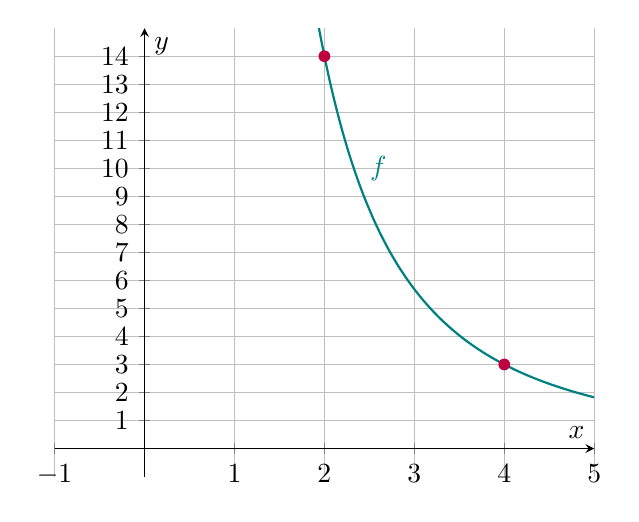
\begin{tikzpicture}
		\begin{axis}[
			axis lines = middle, 
			xmin = -1, xmax = 5,
			ymin = -1, ymax = 15,
			grid = both,
			ytick = {1,2,...,14},
			xlabel = {$x$},
			ylabel = {$y$}
			]
			\addplot[thick, color = teal, samples = 200, domain = 0.4:5]
			{65.333*x^(-2.2224)};
			\node[circle, fill, inner sep = 1.5pt, color = purple] at (axis cs:2,14){};
			\node[circle, fill, inner sep = 1.5pt, color = purple] at (axis cs:4,3){};
			\node[color = teal] at (axis cs:2.6,10) {$f$};
		\end{axis}
	\end{tikzpicture}
	\caption{Graf for potensfunktion $f$.}
	\label{fig:potensopg}
\end{figure}

\begin{enumerate}[label=\roman*)]
	\item Bestem en forskrift for $f$ ved at bruge topunnktsformlen for potensfunktioner
	\item Bestem $f(3)$ og undersøg, om dette passer med Figur \ref{fig:potensopg}.
	\item Løs ligningen $f(x) = 12$.
\end{enumerate}




\subsection*{Opgave 3 (Med Maple)}
\begin{enumerate}
	\item Potensfunktionen $f(x) = 2\cdot x^a$ går gennem punktet $(2,18)$. Brug dette til at bestemme $a$.
	\item Potensfunktionen $f(x) = b\cdot x^1$ går gennem punktet $(3,3)$. Brug dette til at bestemme $b$.
\end{enumerate}

\subsection*{Opgave 4 (Med Maple)}
Det antages, at bremselængden som funktion af hastigheden for en bil er en potenssammenhæng. For en bestemt bil er bremselængden ved 80km/t på 27.4 meter. Ved hastigheden 95km/t er bremselængden 38.7 meter.
\begin{enumerate}[label=\roman*)]
	\item Bestem en potensfunktion der beskriver bremselængden for bilen som funktion af tiden.
	\item Hvad vil bremselængden være for en bil, der kører 130km/t?
	\item Hvor stærkt skal man køre, hvis bremselængden skal være på 200m?
\end{enumerate}

\subsection*{Opgave 5 (Bevis)}
Vi skal besvise topunktsformlen for potensfunktioner. Vi bruger følgende delopgaver til at nå gennem beviset.
\begin{enumerate}[label=\roman*)]
	\item Lav en tegning som på Figur \ref{fig:topunkt} og opskriv forskriften for en potensfunktion $f$.
	\item Indsæt de to punkter i forskriften for $f$, som vi har gjort i begge topunktsformel-beviser fra 
	tidligere for at få et udtryk for $y_1$ og et udtryk for $y_2$
	\item Dividér udtrykket for $y_2$ med udtrykket for $y_1$. Er der noget, der kan forkortes ud?
	\item Brug regnereglen
	\begin{align*}
		\left(\frac{x}{y}\right)^a = \frac{x^a}{y^a}
	\end{align*}
	til at omskrive jeres udtryk.
	\item Tag nu titalslogaritmen af begge sider af lighedstegnet.
	\item Anvend regnereglen 
	\begin{align*}
		\log_{10}(a^x) = x\log_{10}(a)
	\end{align*}
	til at omskrive jeres udtryk.
	\item Isolér $a$ i udtrykket.
	\item Anvend til sidst regnereglen 
	\begin{align*}
		\log_{10}\left(\frac{a}{b}\right) = \log_{10}(a)-\log_{10}(b)
	\end{align*}
	til at omskrive udtrykket. Sammenlign jeres udtryk for $a$ med det fra sætningen. 
	\item Betragt udtrykket for $y_1$ fra punkt ii) og isolér $b$ i dette udtryk.
	\item Sæt en lille, sort firkant, læn dig tilbage og fryd dig.
\end{enumerate} 